
\newglossaryentry{X}
{
  type=genericmath,
  name={$\ensuremath{X} $},
  description={Set of locations for a user. ($R^2$)},
}
\newglossaryentry{Z}
{
  type=genericmath,
  name={$\ensuremath{Z} $},
  description={For every $x \in X$ a perturbed location $z \in Z$ is reported.},
}
\newglossaryentry{privacy level}
{
  type=genericmath,
  name={$\ensuremath{l} $},
  description={Privacy level},
}
\newglossaryentry{radius}
{
  type=genericmath,
  name={$\ensuremath{r} $},
  description={Radius},
}
\newglossaryentry{Epsilon}
{
  type=genericmath,
  name={$\ensuremath{\epsilon} $},
  description={Defined as $\epsilon = l/r$},
}
\newglossaryentry{theta}
{
  type=genericmath,
  name={$\ensuremath{\theta} $},
  description={Angle},
}
\section{2D-Laplace}
The theory for this subject is heavily inspired by the paper that was written by Andrés et al. \citep{DBLP:journals/corr/abs-1212-1984}.
This notion of geo-indistinguishability was introduced to solve the issue of privacy and location data.
It offers an alternative approach for differential privacy by adding noise to the location locally before sending it to a location-based system (LBS) like Google maps.
This section starts with an introduction to mathematics for the planar and polar Laplace algorithm.
For each of the different subsections, we visualize and explain open challenges and theoretic for applying them for clustering.
\glsaddall
\leading{10pt}
\printglossary[type=genericmath, nonumberlist]

\subsection{Planar and polar Laplace}
\printglossary[type=2dlaplace]

The idea of planar Laplace is to generate an area around $x0 \in X$ according to the multivariate Laplace distribution \todo{Link}.
The mechanism of planar Laplace is a modification of the Laplace algorithm to support distance \citep{DBLP:journals/corr/abs-1212-1984}.
This distance method $dist(x, x_`')$ is defined as the Euclidean distance \todo{Link} between two points or sets.
Recalling the definition of Laplace, this method $|x-x_`|$ is replaced by the distance metric.
Hence, the definition of the Probability Density Function (pdf) by Andrés et al. is:
\begin{equation}
  \frac{\epsilon^2}{2*\pi}e(-\epsilon d(x_0, x))
\end{equation}
Which is the likelihood a generated point $z \in Z$ is close to $x0$.
The method works for Cartesian coordinates but was modified to support polar coordinates by including $\theta$.
So each point is reflected as $(r, \theta)$ and can be modified by using a slight modification to work for polar Laplace.
\newpage
A point $z \in Z$ where $z = (r, \theta)$ is randomly generated using two separate methods.
\begin{figure}[h]
  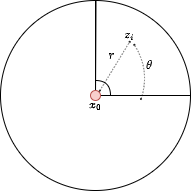
\includegraphics[scale=0.6]{TheorethicalFramework/ND-Laplace/Images/polar-laplace.png}
  \centering
  \caption{Representation of the generated $z = {r \theta}$ and original point $x0$.}
\end{figure}

\textbf{Calculating $r$:}
This variable is described as $dist(x_0, z)$ and can be randomly drawn by inverting the CDF (\textbf{Link}) for the Laplace distribution:
\begin{equation}
  C{_\epsilon}{^{-1}}(p) = - \frac{1}{\epsilon}(W_-1 (\frac{p - 1}{e}) + 1)
\end{equation}
For this equation, $W_-1$ is a Lambert W function with -1 branch.
The Lambert w function, also called the product logarithm is defined as $W(x)e^{W(x)} = x$ \citep{lehtonen_lambert_2016}.
The purpose of the Lambert w function is to invert the CDF of the Laplace distribution to generate random noise for one of the coordinates ($r$) using the random value of $p$.

\textbf{Calculating $\theta$:}
The other coordinate ($\theta$) is defined as a random number $[0, 2\pi]$. \newline \newline
To visualize these methods it is necessary to convert the polar coordinates for $z = (r, \theta)$ back to a plane $(x, y)$.
This is described as step 4 of the planar Laplace algorithm \citep{DBLP:journals/corr/abs-1212-1984} and visualized using figure 1.
\begin{figure}[h]
  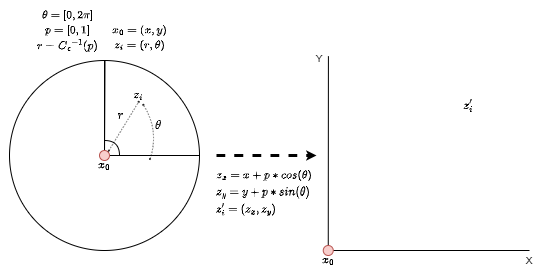
\includegraphics[width=0.8\textwidth]{TheorethicalFramework/ND-Laplace/Images/polar-laplace-to-planar.png}
  \centering
  \caption{Representation of converting the perturbed point $z = (r, \theta)$ to a point ${z_x, z_y}$}
\end{figure}

%% If we want to know if a point is within the radius, 
\subsection{Truncation}
\subsection{Optimizing for clustering}
